\section{Adatmodellek és fő entitások}

A WatchDB jelenlegi MVP verziójának adatmodellje egyszerű, mert a rendszer nem saját filmadatbázist épít. A filmek részletes adatai külső forrásból, a TMDB API-ból érkeznek, az alkalmazás saját adatbázisa pedig elsősorban a felhasználóhoz kötött állapotokat tárolja. Ennek megfelelően a legfontosabb entitások a felhasználó, a watchlist elem, a megnézett film bejegyzés és a külső film entitás.

A felhasználó és a watchlist között egy-a-több kapcsolat van: egy felhasználó több filmet is elmenthet későbbi megtekintésre. Egy adott film egy felhasználó watchlistjén csak egyszer szerepelhet, amit a \texttt{user\_id} és a \texttt{tmdb\_movie\_id} párosa azonosít.

A megnézett filmek külön \texttt{watched} bejegyzésként jelennek meg. A \texttt{rating} mező a felhasználó személyes értékelését tárolja 1 és 5 közötti értékként. A \texttt{watched\_at} opcionálisan azt jelöli, hogy a felhasználó mikor nézte meg a filmet, míg a \texttt{logged\_at} a naplózás időpontját rögzíti. Amikor egy film megnézettként kerül mentésre, a rendszer a hozzá tartozó watchlist bejegyzést eltávolítja.

Fontos tervezési döntés, hogy a WatchDB nem tárolja el a filmek teljes metaadatait saját adatbázisban. A \texttt{tmdb\_movie\_id} mező logikai kapcsolatot teremt a felhasználói adatok és a TMDB filmadatok között. Ennek előnye, hogy az adatmodell egyszerű marad, és nem szükséges saját filmkatalógust karbantartani. Hátránya, hogy a filmcímek, poszterek és egyéb részletek megjelenítése a külső API elérhetőségétől függ.

\begin{figure}[H]
\centering
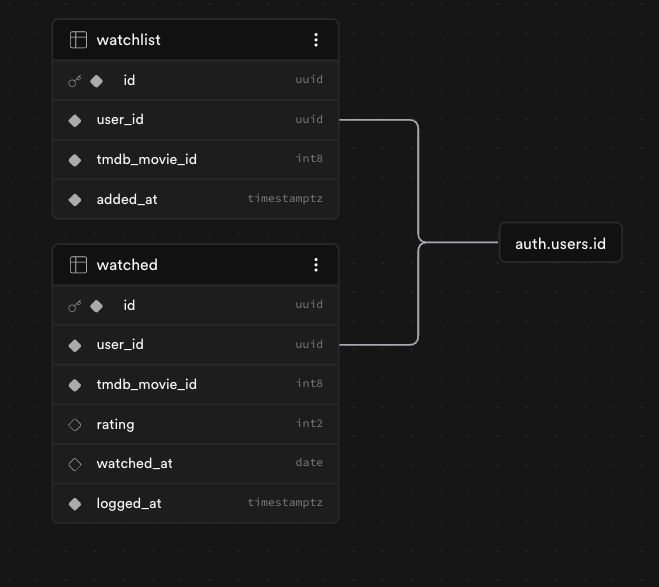
\includegraphics[width=0.85\textwidth]{chapters/chapter-5-systemSpecs/db-schema.png}
\caption{A WatchDB adatbázissémája}
\label{fig:watchdb-db-schema}
\end{figure}

A külső filmadatok a TMDB API-ból érkeznek. Egy részletes filmlekérés eredménye többek között a film azonosítóját, címét, leírását, poszter- és háttérképének elérési útját, megjelenési dátumát, játékidejét, értékelési adatait, státuszát, eredeti nyelvét és műfajait tartalmazza. A külső API válasza a TMDB mezőneveit követi, például \texttt{poster\_path}, \texttt{backdrop\_path}, \texttt{release\_date}, \texttt{vote\_average}, \texttt{vote\_count} és \texttt{original\_language}. Az alkalmazás ezt nem változatlan formában adja tovább, hanem egy belső, JavaScript környezetben természetesebb, camelCase mezőneveket használó objektummá alakítja.

\begin{figure}[H]
\centering
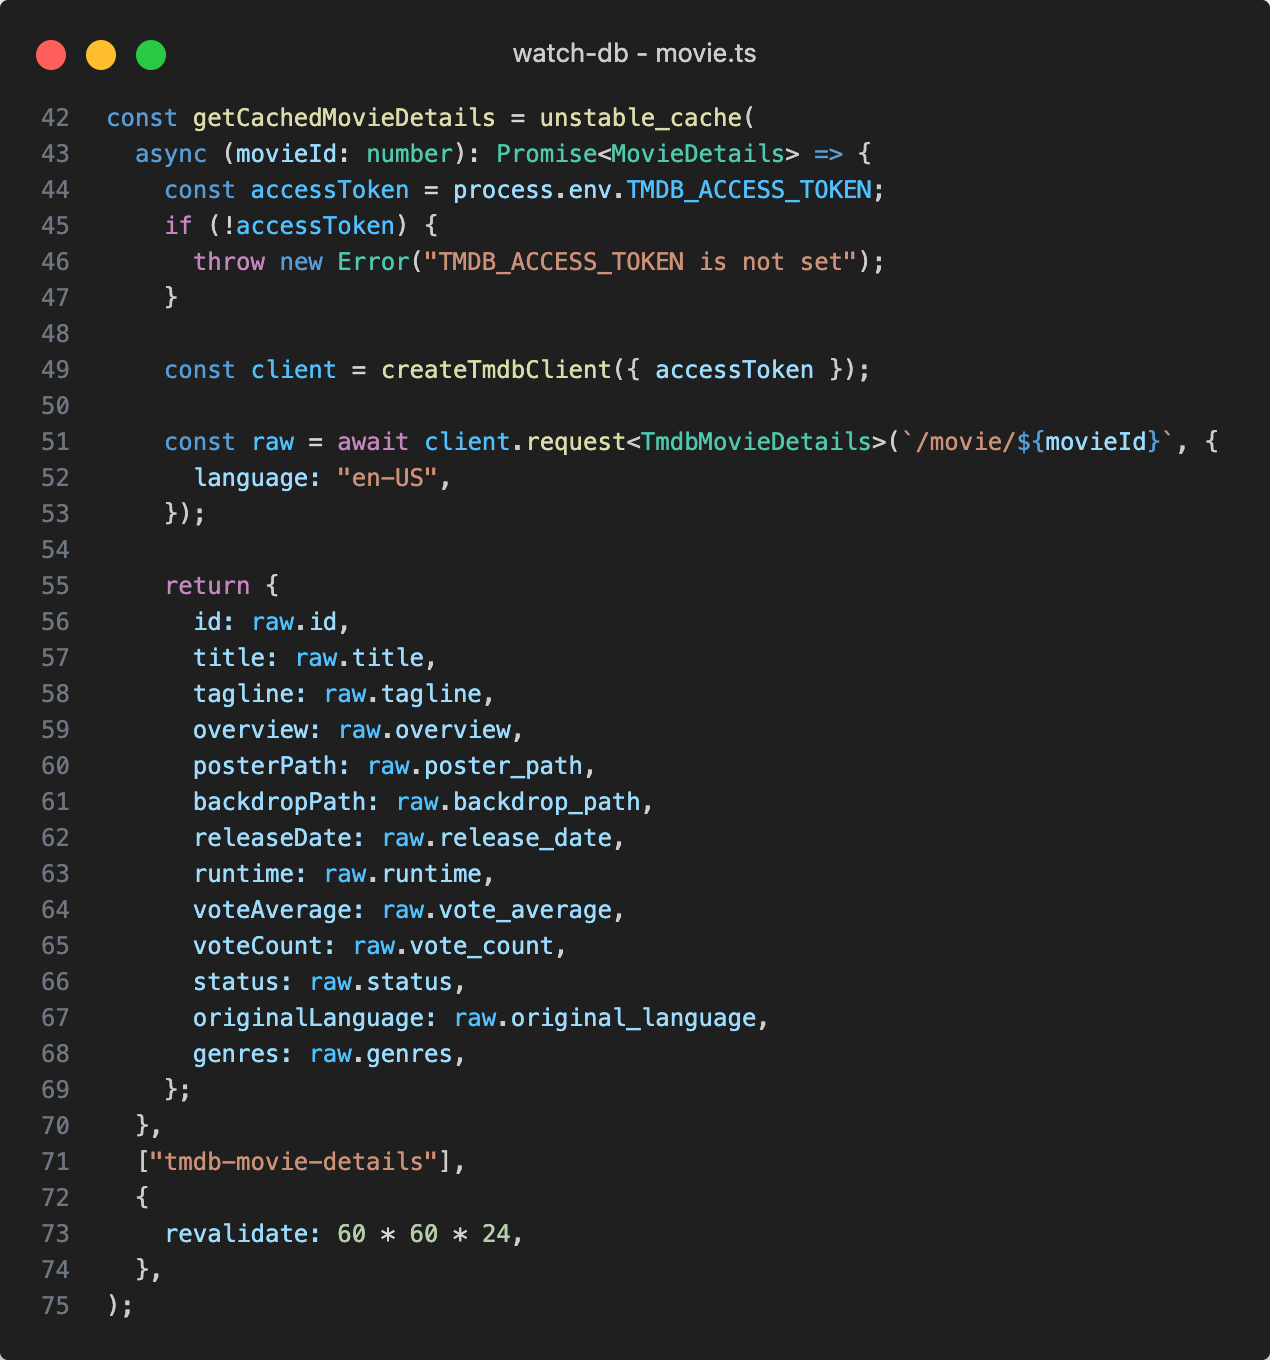
\includegraphics[width=0.95\textwidth]{chapters/chapter-5-systemSpecs/get-cached-movie-details-snippet.png}
\caption{A TMDB filmadatok lekérése és normalizálása}
\label{fig:tmdb-movie-normalization-snippet}
\end{figure}

A kódrészletben az alkalmazás lekéri a film részletes adatait a TMDB API-ból, majd a kapott nyers választ egy belső \texttt{MovieDetails} objektummá alakítja. Ennek során a külső API snake\_case mezőnevei egységes camelCase mezőnevekké válnak, például a \texttt{poster\_path} mezőből \texttt{posterPath}, a \texttt{release\_date} mezőből pedig \texttt{releaseDate} lesz.


\begin{figure}[H]
\centering
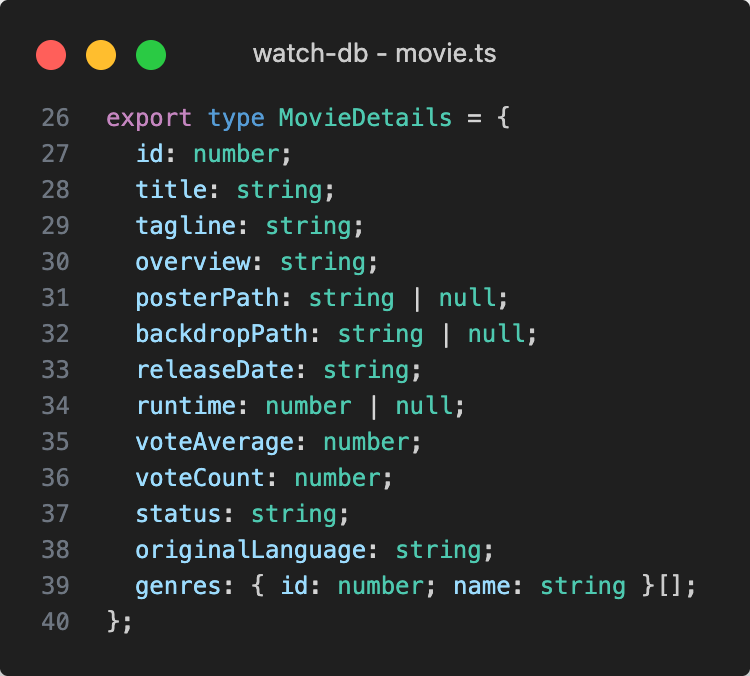
\includegraphics[width=0.55\textwidth]{chapters/chapter-5-systemSpecs/movie-detail-type.png}
\caption{A MovieDetails típusdefiníciója}
\label{fig:movie-details-type}
\end{figure}

Ugyanez az elv jelenik meg a keresési találatoknál is, de ott az alkalmazás szűkebb adatmodellt használ. A keresési lista csak azokat a mezőket tartja meg, amelyek a találati listához szükségesek: az azonosítót, címet, leírást, posztert, megjelenési dátumot és külső értékelési átlagot. A profiloldalon megjelenő watchlist és watched listák ennél is tovább szűkítik az adatot: a TMDB-ből lekért filmcím és poszter mellé csak a saját adatbázisból származó felhasználói állapot kerül, például a hozzáadás ideje, az értékelés vagy a megtekintés dátuma.
